\documentclass{standalone}
\usepackage{tikz}
\usepackage{ctex,siunitx}
\setCJKmainfont{Noto Serif CJK SC}
\usepackage{tkz-euclide}
\usepackage{amsmath}
\usepackage{wasysym}
\usetikzlibrary{patterns, calc}
\usetikzlibrary {decorations.pathmorphing, decorations.pathreplacing, decorations.shapes,}
\begin{document}
\small
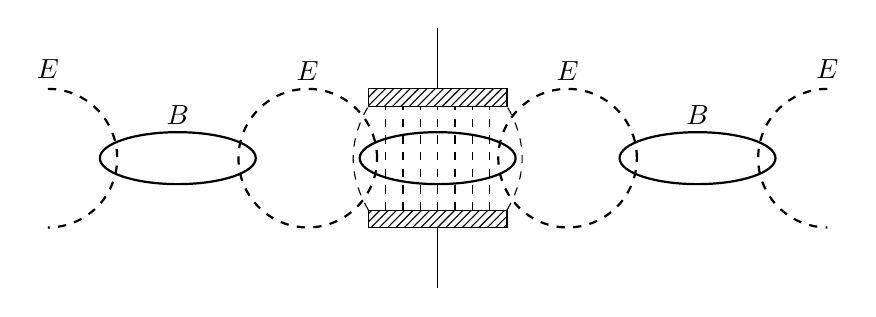
\begin{tikzpicture}[>=latex,scale=1.1]
  % \useasboundingbox(0.9,0)rectangle(5.1,5);
	\draw[pattern=north east lines](-.8,-.8) rectangle (.8,-.6);
	\draw[pattern=north east lines](-.8,.8) rectangle (.8,.6);
	\draw(0,.8)--(0,1.5);
	\draw(0,-.8)--(0,-1.5);
	\foreach \x in {0,3,-3}
	{
		\draw[thick](\x,0) ellipse [x radius=.9, y radius=.3];
	}
	\foreach \x in {1.5,-1.5}
	{
		\draw[dashed, thick](\x,0) circle (.8);
		\node at (\x,1){$E$};
	}
	\draw[dashed, thick](4.5,.8)node[above]{$E$} arc (90:270:.8);
	\draw[dashed, thick](-4.5,.8)node[above]{$E$}  arc (90:-90:.8);
	\foreach \x in {-.6,-.4,-.2,...,.4,.6}
	{
		\draw[dashed](\x,-.6)--(\x,.6);
	}
	\node at (3,.5){$B$};
	\node at (-3,.5){$B$};
	\draw[dashed](-.8,-.6)[bend left=30] to (-.8,.6);
	\draw[dashed](.8,-.6)[bend left=-30] to (.8,.6);
\end{tikzpicture}
\end{document}